\documentclass[12pt]{article}

\author{Pablo Vargas Bermúdez}

\usepackage{minted}
\usepackage[margin=3cm]{geometry}
\usepackage{graphicx}
\usepackage{pdfpages}

\begin{document}
\pagestyle{empty}

\inludepdf[pages=-]{Portada}

\section*{Planteamiento}

Programa que muestra 2 Jlist con al menos 15 colores, los colores
deberán estar dentro de una Enumeración con los atributos RGB. Al
seleccionar un color de la lista deberá de modificar el color de
frente o del fondo del área de prueba.

Use un solo escucha para las 2 listas.

\section*{Código}

\subsection*{Clase Gui}

\inputminted{Java}{Gui.java}

\subsection*{Clase de prueba}

\inputminted{Java}{Prueba.java}

\section*{Ejecución}

\begin{figure}[ht]
  \centering
  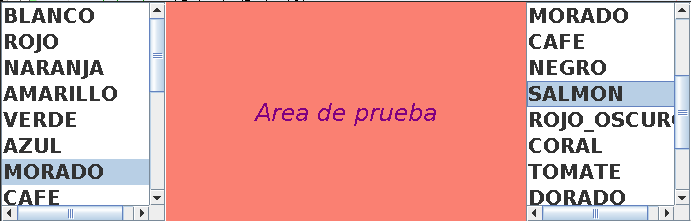
\includegraphics[width=\textwidth]{figures/run1.png}
  \caption{Primera prueba}
\end{figure}

\begin{figure}[ht]
  \centering
  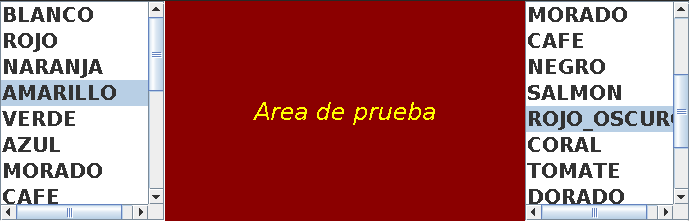
\includegraphics[width=\textwidth]{figures/run2.png}
  \caption{Segunda prueba}
\end{figure}

\begin{figure}[ht]
  \centering
  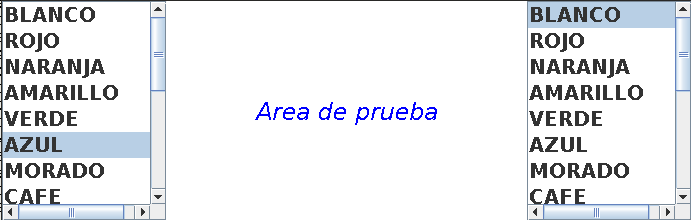
\includegraphics[width=\textwidth]{figures/run3.png}
  \caption{Tercera prueba}
\end{figure}


\end{document}
